\chapter{La ruina del jugador}\label{chap:manual}

\section{Demostración de la ruina del jugador}
http://www.columbia.edu/~ks20/stochastic-I/stochastic-I-GRP.pdf


http://www.ifp.illinois.edu/~sgorant2/gambler.html


Two gamblers Alice and Bob play the following game: Alice repeatedly tosses a fair coin. 
After each toss that comes up H, Bob pays Alice one dollar. After each toss that comes up T, 
Alice pays Bob one dollar. The game continues until either one or the other gambler runs out o
f money. If Alice starts with \$A and Bob starts with \$B,
. What is the probability that, when the game ends, Alice has all the cash?
. What is the expected duration of the game?
 
== Solution
Lets solve the problem using the Doob's Optional stopping Theorem for martingales.
Let $X_1,X_2,\cdots$ be the increments of Alice's wealth. Hence $X_i= 1$, depending on H or T. 
Hence, change in Alice's cash is
\( 
S_n = \sum_{i=1}^n X_i 
\)
Define  
\(
\tau = \min\{t: S_t = +B \mbox{ or } S_t = -A \}
\)
Clearly $\tau$ is a stopping time relative to the natural filtration
$\mathcal{F}_n = \sigma(X_1,X_2,X_3,\cdots,X_n)$. 
$\tau' = \tau \wedge n$ is also a stopping time.

=== (1) Probability of Alice winning
The sequence $S_n$ is a martingale relative to the natural filtration $\mathcal{F}_n$. 
Hence, using Optional Stopping Theorem for $n < \infty$,
\( 
 0 = {E}[S_0] = {E}[S_{\tau \wedge n}] = -A P(\tau \leq n \mbox{ and } S_{\tau} = -A) + B P(\tau \leq n \mbox{ and } S_{\tau} = +B) + E[S_n \chi_{\tau > n}]
 \)                                               
 As $n \to \infty$, the probability that  $\tau > n$ converges to zero. 
 The last term in the above equation is the expectation of a bounded martingale $S_n$
 bounded between $A$ and $B$ and converges to 0. Thus,
 \(
  0 = - A P(S_{\tau} = -A) + B P(S_{\tau} = +B) 
 \)
 Hence, probability that Alice has all the cash $S_{\tau} = +B$ is
 \(
 P(S_{\tau} = +B) = \frac{A}{A+B}.
 \)
 
=== (2) Expected duration of game.
The sequence $(S_n^2-n)$ is a martingale relative to the natural filtration $\mathcal{F}_n$.
Hence, using Optional Stopping Theorem for $n < \infty$,
\( 
 0 = {E}[S^2_0] = {E}[S_{\tau \wedge n}^2 - (\tau \wedge n)]
 \)                                                                                                          
 As $n \to \infty$, the probability that  $\tau > n$ converges to zero. 
Hence,
\(
E[\tau] = E[S_{\tau}^2] = A^2  P(S_{\tau} = -A) + B^2  P(S_{\tau} = +B) = AB 
\)                               
Hence, the expected duration of the game is AB.


 \section{Decidir a favor de quien apostar}
\label{apostar-a-quien}
 \begin{enumerate}[(a)]
  \item Sean $p_L$, $p_z$, $p_v$ las probabilidades de que gane local, empaten o gane visitante, respectivamente. Sean $\mu_L$, $\mu_z$ y $\mu_v$ los momios respectivos. El problema de decisión de apostar \$\,1 en esta situación es:\\
 
 % Set the overall layout of the tree
 \tikzstyle{level 1}=[level distance=3.5cm, sibling distance=2.5cm]
 \tikzstyle{level 2}=[level distance=3.5cm, sibling distance=2cm]
 \tikzstyle{level 3}=[level distance=3.5cm, sibling distance=2cm]


 \begin{figure}[ht]
 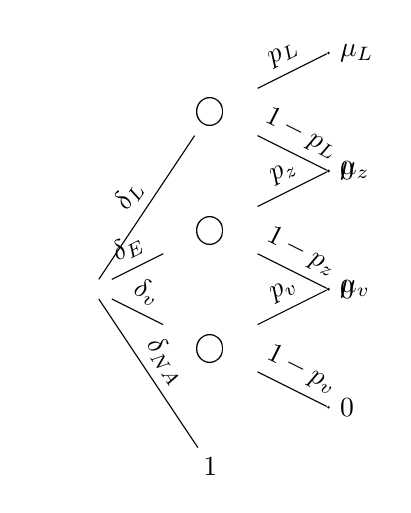
\begin{tikzpicture}[grow=right, sloped]
 \node[text width=4em, text centered] {$\square$}
 %%%%%%%%%%%%%%%%%%%%%%%%%%%%%%%%%%%%%%%%%%%%%%%%%
 %cuarto
 %%%%%%%%%%%%%%%%%%%%%%%%%%%%%%%%%%%%%%%%%%%%%%%%
 child {       
     node[text width=4em, text centered] {1}
              edge from parent         
  node[above] {$\delta_{NA}$}
     }
 %%%%%%%%%%%%%%%%%%%%%%%%%%%%%%%%%%%%%%%%%%%%%%%%%
 %tercero
 %%%%%%%%%%%%%%%%%%%%%%%%%%%%%%%%%%%%%%%%%%%%%%%%
 child {       
     node[text width=4em, text centered] {\textbigcircle}
     child {
                 node[circle, minimum width=1pt,fill, inner sep=0pt, label=right:
                     {$0$}] {}
                 edge from parent
                 node[above] {$1-p_v$}             
             }
             child {
                 node[circle, minimum width=1pt,fill, inner sep=0pt, label=right:
                     {$\mu_v$}] {}
                 edge from parent
                 node[above] {$p_v$}              
             }
              edge from parent         
  node[above] {$\delta_v$}
     }
 %%%%%%%%%%%%%%%%%%%%%%%%%%%%%%%%%%%%%%%%%%%%%%%
 %segundo
 %%%%%%%%%%%%%%%%%%%%%%%%%%%%%%%%%%%%%%%%%%%%%%%%
     child {       
     node[text width=4em, text centered] {\textbigcircle}
     child {
                 node[circle, minimum width=1pt,fill, inner sep=0pt, label=right:
                     {$0$}] {}
                 edge from parent
                 node[above] {$1-p_z$}             
             }
             child {
                 node[circle, minimum width=1pt,fill, inner sep=0pt, label=right:
                     {$\mu_z$}] {}
                 edge from parent
                 node[above] {$p_z$}              
             }
              edge from parent         
  node[above] {$\delta_E$}
     }
 %%%%%%%%%%%%%%%%%%%%%%%%%%%%%%%%%%%%%%%%%%%%%%%
 %primero
 %%%%%%%%%%%%%%%%%%%%%%%%%%%%%%%%%%%%%%%%%%%%%%%%
     child{
     node[text width=4em, text centered] {\textbigcircle}        
             child {
                 node[circle, minimum width=1pt,fill, inner sep=0pt, label=right:
                     {$0$}] {}
                 edge from parent
                 node[above] {$1-p_L$}             
             }
             child {
                 node[circle, minimum width=1pt,fill, inner sep=0pt, label=right:
                     {$\mu_L$}] {}
                 edge from parent
                 node[above] {$p_L$}              
             }    
  edge from parent         
  node[above] {$\delta_L$}
     };  
 \end{tikzpicture}
 \caption{Decidir por quién apostar}
 \end{figure}

   $E_p[U(\delta_i)]=p_i\mu_i;\quad i=L,Z,V$\\
  
   Sol: Se escoge $\rho_i \,\, \cdot \ni \cdot \,\, E_p[U(\delta_i)]=max\{p_L\mu_L,p_z\mu_z,p_v\mu_v,1\}$
  
   \item Se quiere decidir si apostar o no en la ocurrencia de un evento: Sea $p=p(E)$ y $f_p$ densidad de $p$. Sea $\mu$ el momio en el caso de ocurrencia. El problema de decisión asociado es el siguiente:\\
 
 \begin{figure}[!ht]
  \begin{tikzpicture}[grow=right, sloped]
 \node[text width=4em, text centered] {$\square$}
 %%%%%%%%%%%%%%%%%%%%%%%%%%%%%%%%%%%%%%%%%%%%%%%%%
 %segundo
 %%%%%%%%%%%%%%%%%%%%%%%%%%%%%%%%%%%%%%%%%%%%%%%%
 child {       
     node[text width=4em, text centered] {0}
              edge from parent         
  node[above] {$\delta_{NA}$}
     }
 %%%%%%%%%%%%%%%%%%%%%%%%%%%%%%%%%%%%%%%%%%%%%%%
 %primero
 %%%%%%%%%%%%%%%%%%%%%%%%%%%%%%%%%%%%%%%%%%%%%%%%
     child{
     node[text width=4em, text centered]{\textbigcircle}
    	    child {
    	        node[]{\textbigcircle}   	                 
                 %node[above] {$f_p$}
                 child{node[circle, minimum width=1pt,fill, inner sep=0pt, label=right:
                     {$-1$}] {}                    
                 edge from parent
                 node[above] {$1-p$}             
             }
             child {
                 node[circle, minimum width=1pt,fill, inner sep=0pt, label=right:
                     {$\mu-1$}] {}
                 edge from parent
                 node[above] {$p$}              
             }
             edge from parent
             node[above] {$f_p$}}    
  edge from parent         
  node[above] {$\delta_A$}
     };
 \end{tikzpicture}  
 \caption{Decidir si apostar o no apostar}
 \end{figure}
 
 \newpage
  
   $\rightarrow E_p[U(\delta_A)]=E_{f_p}[p(\mu-1)-(1-p)]\\
   =E_{f_p}[p(\mu)-1]\\
   =E_{f_p}(p)\mu-1$\\

   Apuestas si $E_{f_p}(P)\cdot \mu \ge 1$
  
   \item Mismo problema que el caso anterior, sólo que la utilidad depende de $p$ y $\mu$: $U: \Re\times[0,1]\rightarrow\Re$\\
   $(U(0,p)=0\quad\forall p)$.\\
 
 \begin{figure}[ht]
 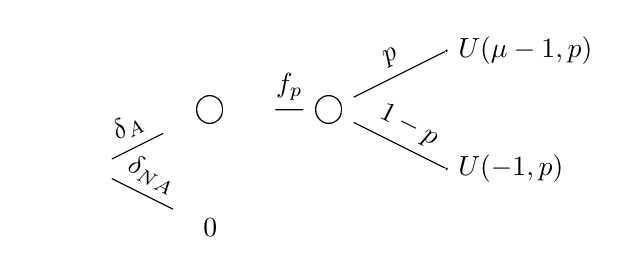
\begin{tikzpicture}[grow=right, sloped]
 \node[text width=4em, text centered] {$\square$}
 %%%%%%%%%%%%%%%%%%%%%%%%%%%%%%%%%%%%%%%%%%%%%%%%%
 %segundo
 %%%%%%%%%%%%%%%%%%%%%%%%%%%%%%%%%%%%%%%%%%%%%%%%
 child {       
     node[text width=4em, text centered] {0}
              edge from parent         
  node[above] {$\delta_{NA}$}
     }
 %%%%%%%%%%%%%%%%%%%%%%%%%%%%%%%%%%%%%%%%%%%%%%%
 %primero
 %%%%%%%%%%%%%%%%%%%%%%%%%%%%%%%%%%%%%%%%%%%%%%%%
     child{
     node[text width=4em, text centered]{\textbigcircle}
    	    child {
    	        node[]{\textbigcircle}   	                 
                 %node[above] {$f_p$}
                 child{node[circle, minimum width=1pt,fill, inner sep=0pt, label=right:
                     {$U(-1,p)$}] {}                    
                 edge from parent
                 node[above] {$1-p$}             
             }
             child {
                 node[circle, minimum width=1pt,fill, inner sep=0pt, label=right:
                     {$U(\mu-1,p)$}] {}
                 edge from parent
                 node[above] {$p$}              
             }
             edge from parent
             node[above] {$f_p$}}    
  edge from parent         
  node[above] {$\delta_A$}
     };
 \end{tikzpicture}
 \caption{Decidir si apostar en función de una utilidad}
 \end{figure}

  
  
   Se apuesta si: \\
   $E_p(U(\delta_A))=E_p[p\,U(\mu-1,p)+(1-p)U(-1,p)]\ge0$
 \end{enumerate}

 Algunas funciones de utilidad posibles:
 \begin{itemize}
  \item $U_\mu(x,p)=x(\frac{1}{\mu}-p)^2$\\
 
  Notese que: $p\,U_\mu(\mu-1,p)+(1-p)U_\mu(-1,p)$\\
 
  $(\hat p=\frac{1}{\mu})=(\hat p-p)^2(p\mu-1)$\\
 
  Me duele más mientras más alejado esté de un trato beneficioso y me produce mayor placer mientras mayor sea el beneficio del trato.
 
  \item $U_{\mu,a}(x,p)= \left\{ \begin{array}{lcc}
              ax(\hat p-p)^2 &   si  & p \le \hat p \\
              & &\\
              x (\hat p-p)^2 &  si & p>\hat p\\             
              \end{array}
  \right.$
 
  Notese que: \\
  \[U_\mu=U_{\mu,1}\]\\
  \[p\,U_{\mu,a}(\mu-1,p)+(1-p)U_\mu(-1,p)= \left\{ \begin{array}{lcc}
              a(\hat p-p)^2 (p\mu-1)&   si  & p \le \hat p \\
              & &\\
              (\hat p-p)^2(p\mu-1) &  si & p>\hat p\\             
              \end{array}
  \right.\]

  Me duele ``a'' veces más un trato perjudicial  que un trato beneficioso si me encuentro a la mis ma distancia que $\hat p$.
 
  \item $U_{\mu,a,b}=U_{\frac{\mu}{1+\mu b},a}$\\
 
  y considerar el problema de decisión con $\mu'=\frac{\mu}{1+\mu b}$.\\
 
  Si $\mu'=\frac{\mu}{1+\mu b}\rightarrow \hat p'=\hat p+b$.\\
 
  Los tratos empiezan a ser beneficiosos hasta que el menos sea $b\%$ más probable que ocurra el evento de lo que sería justo.\\
 
  {\bf Nota:} En un problema de decisión sin aversión a la distribución de probabilidades (o con probabilidades fijas) si se desea apostar en apuestas con un mínimo de ganancias esperadas igual a $b\%$ se debe comparar $\mu_p$ con $1+b$ (i.e. apostar $\leftrightarrow \mu_p \ge 1+b$).
 
 \end{itemize}

 \section{Decidir la cantidad de dinero a apostar}
 \label{sec:cantidad-apostar}

 Supongamos que $\mu_p \ge 1$ y que existen 2 funciones de utilidad:
 \[U_1:\Re^+ \rightarrow \Re^+\]
 \[U_2:\Re^+ \rightarrow \Re^+\]

 La primera es la función de utilidad del dinero para las ganancias y la segunda es la utilidad del dinero para las pérdidas monetarias.\\

 Se harán las siguientes supuestos:

 \begin{enumerate}[(i)]
  \item $U_1(0)=U_2(0)=0$. $U_1$, $U_2$ no decrecientes, una vez cont. dif.
  \item $U'_1(0)>U'_2(0)$ (por lo tanto convendrá apostar).
  \item $\forall M>0$ fija $\displaystyle \lim_{x\rightarrow \infty} \frac{U_1(\mu x)}{U_2(x)}=0$.\\
  (Perder duele muchisimo más que ganar).
 \end{enumerate}
 El problema de decisión asociado a  determinar la cantidad óptima a postar es:(con $0<p<1$ fija y $\mu$ momio)\\

 \begin{figure}[ht]
  \begin{center}
 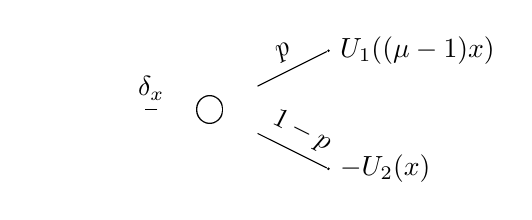
\begin{tikzpicture}[grow=right, sloped]
 \node[text width=4em, text centered] {$\square$}
 %%%%%%%%%%%%%%%%%%%%%%%%%%%%%%%%%%%%%%%%%%%%%%%
 %primero
 %%%%%%%%%%%%%%%%%%%%%%%%%%%%%%%%%%%%%%%%%%%%%%%%
 child{
     node[text width=4em, text centered] {\textbigcircle}        
             child {
                 node[circle, minimum width=1pt,fill, inner sep=0pt, label=right:
                     {$-U_2(x)$}] {}
                 edge from parent
                 node[above] {$1-p$}             
             }
             child {
                 node[circle, minimum width=1pt,fill, inner sep=0pt, label=right:
                     {$U_1((\mu-1)x)$}] {}
                 edge from parent
                 node[above] {$p$}              
             }    
  edge from parent         
  node[above] {$\delta_x$}
     };
 \end{tikzpicture} 
 \end{center}
 \caption{Árbol de probabilidad 4}
 \end{figure}



 $\rightarrow E_p[U(\delta x)]=pU_1((\mu-1)x)-(1-p)U_2(x)$\\

 Sea $f(x)=E_p[U(\delta x)]$\\

 Encontrar el óptimo es encontrar $x \ge 0$ que resuelva el problema: $\displaystyle \max_{x\ge0}f(x)$\\

 \[f'(x)=p(\mu-1)U'_1((\mu-1)x)-(1-p)U'_2(x)=0\]
 \[\frac{p(\mu-1)}{(1-p)}=\frac{U'_2(x)}{U'_1((\mu-1)x)}\]
 P.d.$$\exists \quad x^* \quad \cdot \ni \cdot \quad \frac{p(\mu-1)}{1-p}=\frac{U'_2(x)}{U'_1(\mu x)}$$

 \begin{enumerate}[(i)]

  \item $f'(0)=p(\mu-1)U'_1(0)-(1-p)U'_2(0)>p(\mu-1)U'_2(0)-(1-p)U'_2(0)$\\
 
  $\,\,\,\quad\quad=U'_2(0)(p\,\mu-1)\ge 0$\\
 
  Con $U_2'(0)\ge 0$ y $p\mu\ge0$\\
  Por tanto $f'(0)>0$
 
  \item $f(0)=0$
  \item $\displaystyle\frac{f(x)}{U_2(x)}=p\displaystyle\frac{U_1((\mu-1)x)}{U_2(x)}-(1-p)$\\
  $\rightarrow \displaystyle \lim_{x\rightarrow\infty}\frac{f(x)}{U_2(x)}=-(1-p)$\\
 
  $\rightarrow \exists \, x\,\,\cdot \ni \cdot \,\, \displaystyle\frac{f(x)}{U_2(x)}=-(1+p)+\varepsilon<0$\\
 
  $\rightarrow \exists\,x\,\,\cdot \ni \cdot \,\,f(x)<0$
  \begin{itemize}
   \item Por $T.V.M.\,\,\,\exists\,\, x'\in(0,x)\,\,\cdot \ni \cdot \,\,xf'(x')=f(x)-f(0)=f(x)<0$\\
   $\rightarrow f'(x')<0$
   \item T.V.I. $\exists\,\, x^*\in(0,x')\,\,\cdot \ni \cdot \,\,f'(x^*)=0$. i.e. $\displaystyle\frac{p(\mu-1)}{1-p}=\displaystyle\frac{U'_2(x)}{U'_1(\mu x)}$\\
  
   Como $f$ es primero creciente y en algún punto decreciente:\\
   $\rightarrow x\,\,\cdot \ni\cdot\,\,f'(x)=0$ es un maximizador.
  \end{itemize}
 \end{enumerate}

 Algunas funciones a considerar:
 \begin{itemize}
  \item $U_{1,\alpha}(x)=x^{\alpha}\qquad\qquad 0<\alpha<1$\\ 
  $U_2(x)=x$\\
 
  Compruébense los supuestos:
  \begin{enumerate}[(i)]
   \item $U_{1,\alpha}(0)=0=U_2(0)$, son crecientes y una vez dif.
   \item $U'_{1,\alpha}(0)=+\infty$, $U'_2(0)=1\qquad{\therefore \,\, U'_{1,\alpha}(0)>U'_2(0)}$
   \item $\forall \,\, \mu>0$\\
  
   $\displaystyle\lim_{x\rightarrow +\infty}\displaystyle\frac{U_{1,\alpha}(\mu x)}{U_2(x)}=\mu^{\alpha}\displaystyle\lim_{x\rightarrow +\infty}\displaystyle\frac{x^{\alpha}}{x}=\mu^{\alpha}\displaystyle\lim_{x\rightarrow +\infty}\displaystyle\frac{1}{x^{1-\alpha}}=0$\\
  
   Para una apuesta con probabilidad $p$ y momio $\mu$ el óptimo se da en:\\
  
   $\displaystyle{\frac{p(\mu-1)}{(1-p)}=\frac{U'_2(x)}{U'_{1,\alpha}((\mu-1)x)}=\frac{1}{\alpha((\mu-1)x)^{\alpha-1}}=\frac{1}{\alpha}(\mu-1)^{1-\alpha}x^{1-\alpha}}$\\\\
  
   $\rightarrow \left(\displaystyle\frac{\alpha p}{(1-p)}\right)(\mu-1)^{\alpha}=x^{1-\alpha}\rightarrow x^*=\left(\displaystyle\frac{\alpha p}{1-p}\right)^{\frac{1}{1-\alpha}}(\mu-1)^{\alpha/1-\alpha}$\\
  \end{enumerate}

  \item $U_{1,\alpha}(x)=x^{\alpha}\qquad\qquad 0<\alpha<1$\\
  $U_{2,\beta}(x)=x^{\beta}\qquad\qquad \beta \le1$\\
 
  Es fácil revisar los supuestos. Para una apuesta con probabilidad $p$ y momio $\mu$ el óptimo se da en:\\
 
  ${\displaystyle\frac{p(\mu-1)}{(1-p)}=\frac{\beta x^{\beta-1}}{\alpha(\mu-1)^{\alpha-1}x^{\alpha-1}}=\frac{\beta}{\alpha}(\mu-1)^{1-\alpha}x^{\beta-\alpha}}$\\
 
  $\rightarrow{\displaystyle\left(\frac{\alpha p}{\beta(1-p)}\right)(\mu-1)^{\alpha}=x^{\beta-\alpha}\rightarrow x^*=\left(\frac{\alpha p}{\beta(1-p)}\right)^{1/\beta-\alpha}(\mu-1)^{\alpha/\beta-\alpha}}$
 
  \item $U_1(x)=\ln (x)$\\
  $U_2(x)=x$\\
 
  Es fácil revisar los supuestos. Para una apuesta con probabilidad $p$ y momio $\mu$ el óptimo se da en:\\
 
  ${\displaystyle \frac{p(\mu-1)}{(1-p)}=\frac{1}{(\frac{1}{(\mu-1) x})}=(\mu-1)x\rightarrow x^*=\frac{p}{1-p}}$\\
 
  \item $U_{1,\alpha}(x)=1-e^{-\alpha x}\qquad\qquad \alpha \ge 1$\\
  $U_2(x)=x$\\
 
  Es fácil revisar los supuestos. Para una apuesta con probabilidad $p$ y momio $\mu$ el óptimo se da en:\\
 
 \[{\displaystyle\frac{p(\mu-1)}{1-p}=\frac{1}{\alpha e^{-\alpha(\mu-1)x}}\,\,\rightarrow \,\,\ln \left(\frac{\alpha p(\mu-1)}{(1-p)}\right)=\alpha(\mu-1)x}\]
 \[\qquad\qquad\qquad\qquad\qquad\qquad\rightarrow\,\, x^*={\displaystyle\frac{1}{\alpha (\mu-1)}\ln \left(\frac{\alpha p(\mu-1)}{(1-p)}\right)}\]
 \end{itemize}

 Otras tres funciones de utilidad a considerar:

 \begin{itemize}
  \item $U_{1,\alpha}(x)=\alpha x \qquad\qquad \alpha \ge 1$\\
  $U_2(x)=e^x-1$\\
 
  $\rightarrow {\displaystyle\frac{p(\mu-1)}{1-p}=\frac{e^x}{\alpha}}$\\
 
  $\rightarrow x^*=\ln \left(\displaystyle\frac{p(\mu-1)}{1-p}\right)+\ln (\alpha)$
 
  \item $U_1(x)=\ln (x)\qquad\qquad \alpha \ge 1$\\
  $U_2(x)=x^{\alpha}$\\
 
  $\rightarrow {\displaystyle\frac{p(\mu-1)}{1-p}=\frac{\alpha x^{\alpha-1}}{\frac{1}{(\mu-1)x}}=\alpha(\mu-1)x^{\alpha}}$\\
 
  $\rightarrow x^*=\left(\displaystyle\frac{p}{\alpha(1-p)}\right)^{1/\alpha}$
 
  \item $U_{1,\alpha}(x)=\tan^{-1}(x)$\\
  $U_{2,\alpha}(x)=\alpha x\qquad\qquad 0<\alpha\le 1$\\
 
  $\rightarrow \displaystyle\frac{p(\mu-1)}{1-p}=\alpha(1+(\mu-1)^2x^2)$\\
 
  $\rightarrow \displaystyle\frac{p\mu-p-\alpha(1-p)}{1-p}=\alpha(\mu-1)^2x^2$\\
 
  $\rightarrow \displaystyle\frac{p\mu-(1-\alpha)p-\alpha}{1-p}=\alpha(\mu-1)^2x^2$\\

  $\rightarrow x^*={\displaystyle\frac{1}{\sqrt{\alpha}(\mu-1)}\left(\frac{p\mu-(1-\alpha)p-\alpha}{1-p}\right)^{1/2}}$\\
 
  equivalentemente:  $x^*={\displaystyle\frac{1}{\mu-1}\left(\frac{p\mu-(1-\alpha)p-\alpha}{1-p}\right)^{1/2}}$\\
 
  Basta probar que $p\mu-(1-\alpha)p-\alpha \ge 0$\\
 
  $p\mu-(1-\alpha)p-\alpha \ge p\mu-(1-\alpha)-\alpha=p\mu-1 >0$\\
 
  $x^*$ está bien definido.
 \end{itemize}
 
 \subsection{Ahorro precaucional}
\label{sec:ahorro-precaucional}
 Supongamos $F_1,...,F_n$ distribuciones y la siguiente sucesión de Variables aleatorias $(x_1^t)_{t=1}^{\infty},..., (x_n^t)_{t=n}^{\infty}$ independientes $x_j^{t} \sim F_j \,\forall\, t\, \in\, \mathbb{N}$.\\

 Sean $\alpha_1,..., \alpha_n\,\in\,\Re^+\,\, \cdot \ni \cdot \,\,\displaystyle \sum_{j=1}^n\alpha_j=1$, definimos:

 \begin{itemize}
  \item $z_1=\displaystyle \sum_{j=1}^n\alpha_jx_j'$
  \item $z_{t+1}=\displaystyle \sum_{j=1}^n\alpha_jx_j^{t+1}+z_t$
 \end{itemize}
 Supongamos que $E[x_j^t]>1\,\,\forall\,t \,\in\,\mathbb{N}\rightarrow E[z_t]=tE[z_1]=t\mu>1$\\

 {\bf Problema:}\\
 Encontrar $y \,\,\cdot \ni\cdot\,\,(1-ty)+yz_t \ge y\,\,\forall\,t\,\in \mathbb{N}$ con probabilidad $(1-\alpha)\times 100\%$. $(y\in[0,1])$.

 $$\rightarrow y z_t\ge (t+1)y-1\quad\rightarrow\quad z_t\ge(t+1)-\frac{1}{y}$$
 $$\qquad\qquad\qquad\qquad\qquad\qquad\qquad\,\,\rightarrow z_t\ge t+k (con\,\,\,k=1-\frac{1}{y})$$

 equivalentemente: Encontrar $k\le 0\,\,\cdot\ni\cdot\,\,z_t\ge t+k\,\,\forall\,t\in\mathbb{N}$ con probabilidad $(1-\alpha)\times 100\%$.\\

 Sol: \\
 Sea $\mu=E[z_1]$, $\sigma^2=Var[z_1]$\\

 \[\rightarrow (1-\alpha)=p(z_t)\ge t+k\,\,\forall\,\in\mathbb{N}\qquad\qquad\qquad\qquad\qquad\qquad\qquad\qquad\quad\quad\]
 \[=p(z_1\ge 1+k)\cdot p(z_2\ge 2+k\,\,|z_1\ge 1+k)\cdots\qquad\quad\]
 \[=p(z_1\ge 1+k)\cdot\displaystyle\prod_{t=1}^{\infty}p(z_{t+1}\ge (t+1)+k\,|z_t\ge t+k)\]\\

 Usando el T.C.L.: $z_t \rightarrow N(t\mu,\,t\sigma^2)\,\,\forall\,t\in\,\mathbb{N}$

 \begin{enumerate}[(i)]
  \item $p(z_1\ge 1+k)=p{\displaystyle\left(\frac{z_1-\mu}{\sigma}\ge\frac{(1+k)-\mu}{\sigma}\right)=1-\Phi\left(\frac{k-(\mu-1)}{\sqrt{t}\sigma}\right)}$\\

  \item $p(z_{t+1}\ge (t+1)+k\,|z_t\ge t+k)=\displaystyle\frac{p(z_{t+1}\ge (t+1)+k,\,z_t\ge t+k)}{p(z_t\ge t+k)}$\\

     \begin{itemize}
      \item $p(z_t\ge t+k)=p{\displaystyle\left(\frac{z_t-t\mu}{\sqrt{t}\sigma}\ge\frac{k-t(\mu-1)}{\sqrt{t}\sigma}\right)}$\\

      $\qquad\qquad\qquad={\displaystyle 1-\Phi\left(\frac{k-t(\mu-1)}{\sqrt{t}\sigma}\right)}$\\

      \item $z_{t+1}=y_t+z_t$ con $y_t \sim (\mu,\sigma^2),\,\,y_t,z_t$ independientes\\ $z_t\sim(t\mu,t\sigma^2)$
     \end{itemize}
 $\rightarrow f(y_t,z_t)\simeq \displaystyle\frac{1}{2\pi\sqrt{t}\sigma^2}\exp\{-\frac{1}{2\sigma^2}[(y_t-\mu)^2+\frac{1}{t}(z_t-t\mu)^2]\}$
 \end{enumerate}

 Sea \[\omega_t=y_t+z_t\qquad\qquad y_t=\omega_t-v_t\]
 %\[\rightarrow\]
 \[v_t=z_t\qquad\qquad z_t=v_t\]

 \[\rightarrow J=\left( {1\atop 0} {-1\atop {1}} \right)\rightarrow |det(J)|=1\]

 \[f(z_{t+1}z_t)=\displaystyle\frac{1}{2\pi\sqrt{t}\sigma^2}\exp\{\displaystyle -\frac{1}{2\sigma^2}[(z_{t+1}-z_t-\mu)^2+\frac{1}{t}(z_t-t\mu)^2]\}\]\\

 $\rightarrow p(z_{t+1})\ge (t+1)+k,\,z_t\ge t+k$\\

 \[={\displaystyle\int_{t+k}^{\infty}\int_{t+1+k}^{\infty}\frac{1}{2\pi\sqrt{t}\sigma^2}\exp\{\displaystyle -\frac{1}{2\sigma^2}[(z_{t+1}-z_t-\mu)^2+\frac{1}{t}(z_t-t\mu)^2]\}}dz_{t+1}dz_t\]\\

 \[{=\displaystyle\frac{1}{2\pi\sqrt{t}\sigma^2}\int_{t+k}^{\infty}\exp\{-\frac{1}{2\sigma^2 t}(z_t-t\mu)^2\}\int_{t+1+k}^{\infty}\frac{1}{\sqrt{2\pi}\sigma}\exp\{\displaystyle -\frac{1}{2\sigma^2}[(z_{t+1}-z_t-\mu)^2\}dz_{t+1}dz_t}\]\\

 \newpage

 \[\footnote{Ver Apéndice A}= {\displaystyle\frac{1}{2\pi\sqrt{t}\sigma^2}\int_{t+k}^{\infty}\exp\{-\frac{1}{2\sigma^2 t}(z_t-t\mu)^2\}\left[1-\Phi\left(\frac{k+t-z_t-(\mu-1)}{\sigma}\right)\right]}\]

  \rule{14cm}{0.1mm}
 \[\overline{z_t}=\frac{1}{t}z_t,\,\,\,d\overline{z_t}=\frac{1}{t}dz_t,\,\,\,(\overline{z_t})_0=1+\frac{k}{t},\,\,\,(\overline{z_t})_1=\infty\]
  \rule{14cm}{0.1mm}

 \[={\displaystyle\frac{\sqrt{t}}{2\pi\sqrt{t}\sigma^2}\int_{1+k/t}^{\infty}\exp\{-\frac{t}{2\sigma^2 }(\overline{z}_t-\mu)^2\}\left[1-\Phi\left(\frac{k+t(1-\overline{z}_t)-(\mu-1)}{\sigma}\right)\right]d\overline{z}_t}\]

 Por tanto:\\

 $p(z_{t+1})\ge (t+1)+k,\,z_t\ge t+k$\\

 \[\simeq {\displaystyle \frac{\sqrt{t}\int_{1+k/t}^{\infty}\exp\{-\frac{t}{2\sigma^2 }(\overline{z}_t-\mu)^2\}\left[1-\Phi\left(\frac{k+t(1-\overline{z}_t)-(\mu-1)}{\sigma}\right)\right]d\overline{z}_t}{\sqrt{2\pi}\sigma\left(1-\Phi\left(\frac{k-t(\mu-1)}{\sqrt{t}\sigma}\right)\right)}}\]

 Para calcular $k$ se resuelve la siguiente ecuación:

 \[\log (1-\alpha)=\log(p|z_1\ge 1+k)+\displaystyle\sum_{t=1}^{\infty}\log(p(z_{t+1})\ge (t+1)+k,\,z_t\ge t+k)\]

 \[y=\frac{1}{1-k}\]

 Se realizó una muestra $y_1,..., y_n$, donde:

 \[y_1=CA(p_i,\mu_i,\sigma_i)\]

 Donde:
 \begin{itemize}
  \item $p_i$: Un valor de probabilidad deseado.
  \item $M_i$: Un valor de $E[z_1]$ dado.
  \item $\delta_i$: Un valorde $Var(z_i)^{1/2}$.
  \item $CA$: La función que se define implícitamente de resolver las ecuaciones para calcular la cantidad de apostar.
 \end{itemize}

 A tales datos se les ajustó el siguiente modelo lineal:

 \[y_i=\beta_0+\beta_1p_i+\beta_2\mu_i+\beta_3\sigma_i+\varepsilon_i\]

 \newpage

 El ajuste es el siguiente:

 \begin{itemize}
  \item $\beta_0=0.2925$
   \item $\beta_1=-0.9975$
  \item $\beta_2=1.3772$
  \item $\beta_3=-1.1127$
 \end{itemize}

 Con $R^2=0.95$.\\

 En adelante, se tomará como aproximación lo siguiente:

 \[CA(p,\mu,\sigma)\simeq0.2925-0.9975p+1.3772\mu-1.1127\sigma\]

 \subsection{Evolución del dinero en el tiempo}
 \label{sec:evolucion-dinero}
 {\bf Problema:} Decidir $p$ de manera óptima.\\

 Sea $x$ la cantidad de ingresos restantes ($o\ge x\ge1$, en porcentaje), y $\mu$, $\sigma$ la media y la desviación estandar de apostar en un periodo dados.\\

 Supongamos $U_1,U_2: \Re^+\rightarrow \Re^+$ funciones de utilidad del dinero. ($U_1$ ganancias, $-U_2$ pérdidas) $\cdot\ni\cdot$ son no decrecientes y una vez continuamente diferenciables. Considerese la siguiente función:\\

 \[f(p;x,\mu,\sigma)=[beneficio]-[costo]\]
 \[f(p;x,\mu,\sigma)=[pU_1(y(p,\mu,\sigma)\mu x)]-[(1-p)U_2(x)]\]\\

 Suponiendo $y(p,\mu,\sigma)=a_0-a_1p+a_2\mu-a_3\sigma$ se obtiene:\\

 $a_i\ge 0,\,\,i=0,...,3$
 \[f=pU_1((a_0-a_1p+a_2\mu-a_3\sigma)\mu x)-(1-p)U_2(x)\]

 El problema es:\\

 $max\,\,f$\\

 Sol:\\

 \[f'(p)=-pU_1'((a_0-a_1p+a_2\mu-a_3\sigma)\mu x)a_1\mu x\]
 \[\qquad\qquad\qquad+U_1((a_0-a_1p+a_2\mu-a_3\sigma)\mu x)+U_2(x)=0\]

 Si $U_1$ es cóncava $\rightarrow$ $p^*$ es un maximizador.\\

  Forma aproximada de obtener $p$ :

  \[y=a_0-a_1p+a_2\mu-a_3\sigma\]

  $\rightarrow$ Sea $b=a_1\mu x$, $p_0$ una aproximación de $p$. Definimos:

  \[\omega=y\mu x,\quad \omega_0=y(p_0,\mu,\sigma)\mu x\]

  \[\rightarrow U_1(\omega)=U_1(\omega_0)+U'_1(\omega_0)(\omega-\omega_0)+O((\omega-\omega_0))\]
  \[=U_1(\omega_0)+bU'_1(\omega_0)(\omega_0)(p-p_0)+O((\omega-\omega_0))\]

  Se puede aproximar $f$ por:

  \[f(p)\simeq p[U_1(\omega_0)+bU'_1(\omega_0)(\omega_0)(p-p_0)]-(1-p)U_2(x)\]

  \[\Rightarrow f'(p)\simeq U_1(\omega_0)-2bU'_1(\omega_0)p+bU'_1(\omega_0)p_0+U_2(x)=0\]

  \[\Rightarrow p\simeq \frac{1}{2bU'_1(\omega_0)}[U_1(\omega_0)+U_2(x)]+\frac{1}{2}p_0\]

 Supongamos $U_1:\Re^+ \rightarrow \Re^+$ dada por $U(\omega)=\omega^\alpha\qquad(0<\alpha\le1)$ y $U_2(x)=\beta x$\\

 Notese que:
 \begin{itemize}
  \item ${\displaystyle\frac{U_1(\omega_0)}{U'_1(\omega_0)}=\frac{\omega_0}{\alpha}}$
  \item ${\displaystyle\frac{\omega_0}{b}=\frac{a_0-a_1p+a_2\mu-a_3\sigma}{a_1}}$
 \end{itemize}

 \[\Rightarrow p\simeq \frac{1}{2\alpha a_1}[a_0+a_2\mu-a_3\sigma+\frac{\beta}{\mu}[(a_0-a_1p_0+a_2\mu-a_3\sigma)\mu x]^{1-\alpha}]+\frac{1}{2}(1-\frac{1}{\alpha})p_0\]

 Supongamos ahora que $f$ es de la siguiente forma:

 \[f(p)=pU_1(y(p,\mu,\sigma)\cdot \mu x)-(1-p)U_2(x)-pU_3(\theta(k\sigma-\mu))\]

 i.e. Hay pérdidas potenciales por el riesgo de la inversión considerar
 \[U_3(\theta(k\sigma-\mu))U_2(\theta(k\sigma-\mu)x)I(\theta(k\sigma-\mu)\ge 0)\]

 $\Rightarrow$ De manera análoga se obtiene:

 \[p\simeq\frac{1}{2bU'(\omega_0)}[U_1(\omega_0)+U_2(x)+U_2(\theta(k\sigma-\mu)xI_{\{m\ge0\}}]+\frac{1}{2}p_0\]

 \newpage
 Si tomamos $U_1(\omega)0\omega^\alpha$, $U_2(x)=\beta x$ \\\\

 $p\simeq \frac{1}{2\alpha a_1}\{(a_0+a_2\mu-a_3\sigma)$
 \[+\frac{\beta_1}{\mu}[1+(\beta_2\sigma-\beta_3 \mu)I_{\{m\ge0\}}][(a_0-a_1p+a_2\mu-a_3\sigma)\mu x]^{1-\alpha}\}+\frac{1}{2}(1-\frac{1}{\alpha})p_0\]

 